\section{Продолжение о распространении волн сферической формы}
\begin{enumerate}
  \item Добавления о потенциале источника в сжимаемой жидкости. Запаздывающий потенциал.
  \item Растространение малых возмущений от движущегося источника. Эффект Доплека. Конус Маха.
  \item Распространение конечных (не малых) возмущений. Пример: волны Римана.
\end{enumerate}

\subsection{Источник в газе (в сжимаемой жидкости)}
Потенциал такой
\[
  \phi = -\frac{Q\left(t - \frac t{a_0}\right)}{4\,\pi\,r};\qquad v = \CP \phi r.
\]
Из этого следуем два вывода. Одни я говорила, а второй не сказала.
Пусть $Q(t)\ne0$ при $0\le t\le t_1$.
\begin{enumerate}
\item В любой момент времени $\phi\ne0$, если $0\le t-\frac r{a_0}\le t_1$. Где он не равен нулю? Во всём пространстве или нет? Неравенство на $r$ получается $a_0(t-t_1)\le  r\le a_0\,t$.
% рисунок одна сфера
Пока источник работает, есть только один фронт передний $a_0\,t$. Если же $t>t_1$ появится задний фронт $a_0(t-t_1)$. Чем больше время, тем тоньше слой между сферами.
% картинка две сферы, источник крестом

А в несжимаемой жидкости потенциал отличен от нуля везде, но только моменты работы источника.

\item В любой точке $r$ $\phi\ne0$, если $\frac r{a_0}\le t\le t_1 + \frac r{a_0}$.
% картинка источник и точка.
Это иструкция по нахождению времени, за которое позмущение дойдёт до заданной точки. Человек слышит источник ровно столько, сколько работает источник, но с запаздыванием.
Ипользуют термин «запаздывающий потенциал» для вот этой формулы
\[
  \phi = -\frac{Q\left(t-\frac r{a_0}\right)}{4\,\pi\,r}.
\]
\end{enumerate}
\subsection{Возмущения от движущегося источника}
\subsubsection{Движение по прямой}
Пусть источник сначала движется по прямой со скоростью $u$. Будем считать, что потенциал источника формируется из набора источников, каждый из которых вспыхивает в тот момент, когда наша точка через него проходит.
\begin{figure}[H]
\centering
  \begin{tikzpicture}
    \draw (-2,0)--(2,0)
	  (-2,-0.1)--(-2,0.1) node [anchor=north]{$t=0$} node[anchor=south]{$M_0$}
	  (0,-0.1)--(0,0.1) node [anchor=north]{$t=t_1$} node[anchor=south]{$M_1$}
	  (1.5,-0.1)--(1.5,0.1) node [anchor=north]{$t$} node[anchor=south]{$M$};
    \draw (3,0) arc (0:360:5cm);
    \draw (2.5,0) arc (0:360:2.5cm);
\end{tikzpicture}
\caption{Источник движется по прямой}
\label{lineIst}
\end{figure}

\begin{enumerate}
\item Пусть $u<a_0$. Возмущения обгоняют источник. Возмущение, которое было послано в момент $t=0$ находится на сфере $a_0\,t>u\,t$. Возмущение, которое возникло при $t=t_1$ в точке $M_1$ "--- на сфере с центром в $M_1$ радиуса $a_0(t-t_1)>u(t-t_1)$. Это не концентрические сферы, это сферы со смещёнными центрами. Если источник движется бесконечно долго, всё пространство и позади и впереди будет возмущено. Если не бесконечно долго, будет передний фронт; если поставить наблюдателя, он услышит источник быстрее, чем сам источник к нему дойдёт.

Как раз в этом случае имеет смысл говорить про эффект Допплера. Открыт Допплером. Про сфет этот эффект лучше заметен, потому что свет всегда движется с досветовой скоростью. Эффект состоит в том, что если источник работает, например, периодически, издаёт звук определённой частоты, и движется, то наблюдатель, к которому этот источник движется, слышит звук более высокой частоты, чем издавал источник, а тот, который позади источника, слышит звук более низкой частоты. (См. Седов «МСС», том 2).

Вычислим, как же меняется частота. Пусть источник $Q(t)$ имеет такой вид
\begin{figure}[H]
\centering
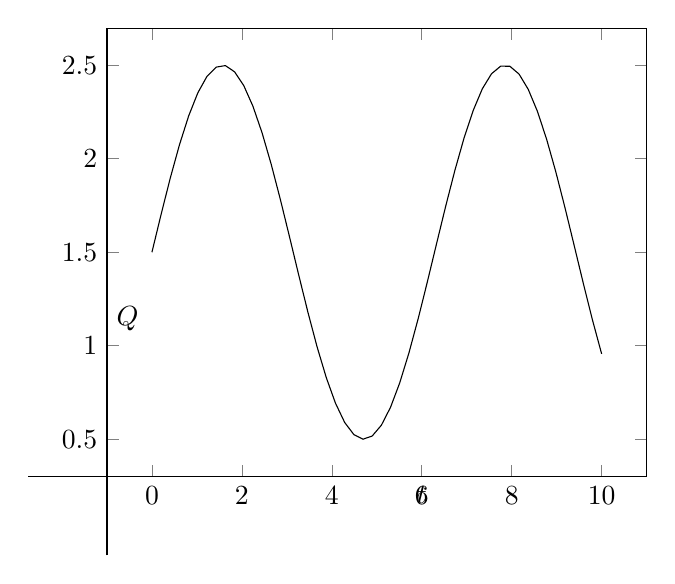
\begin{tikzpicture}
  \draw(-1,0)--(4,0) node[anchor=north]{$t$}
	(0,-1)--(0,2) node[anchor=west]{$Q$};
   \begin{axis}
   \addplot[domain=0:10,samples=50]({x},{1.5+sin((x) r)});
  \end{axis}
\end{tikzpicture}<++>
\caption{<+caption text+>}
\label{fig:<+label+>}
\end{figure}
Пусть $Q(t)$ таков, что $\tau$ "--- период его колебаний по времени. $\w = \frac1\tau$ "--- частота. И есть наблюдатель впереди. Наблюдатель находится на расстоянии $l$ от $M_0$. Тогда
\[
  \tau_{\text{набл}} = \Delta t = \tau +\frac{l-u\tau}{a_0} - \frac l{a_0} = \tau\left(1-\frac u{a_0}\right);\quad \w_{\text{набл}} = \frac1{\tau_{\text{набл}}}.
\]

\item Теперь картина возмущений при $u=a_0$. Передний фронт находится там же, где находится источник. Все сферы имеют в каждый момент общую точку, совпадающую с позицией источника. Если наблюдатель стоит впереди, то он его не слышит. Когда источник придёт, тогда и услышит. А когда источник движется бесконечно долго со звуковой скоростью, то сфера-фронт растягивается в плоскость. Слева от плоскости возмущённая среда, права "--- невозмущённая.

\item $u>a_0$. Источник крикнул и убежал. Тогда радиусы сфер будут меньше расстояния от источника, до центра сферы. Все сферы находятся внутри некоторого конуса.
\begin{figure}[H]
\centering
\begin{tikzpicture}
  \draw(-3,0)--(4,0) node[anchor=south east]{$\alpha$};
  \draw(2.5,0) arc (0:360:2.5cm);
  \draw(0,0)--(1.5,2)--(5.5,-1);
\end{tikzpicture}<++>
\end{figure}<++>
$\alpha$ "--- половина угла Конуса, внутри которого наблюдаются возмущения при сверхзвуковом движении источника. Называется он углом Маха.
\[
  \sin\alpha = \frac{a_0(t-t_1)}{u(t-t_1)} = \frac{a_0}u = \frac1M.
\]
Ну а $M = \frac u{a_0}$ "--- число Маха.

Наблюдатель тем более не слышит источник, когда тот к нему приближается. Если летит сверхзвуковой самолёт, сначала его видите, а потом уже слышите.

Никто не исследует в лаборатории быстро движующийся источник. Источник фиксируют и обтекают сверхзвуковым потоком.
\end{enumerate}

А если источник движется не по прямой и не с постоянной скоростью, то картинки сложнее. Можно рассматривать тонкое крыло, как источник малых возмущений. Фронт уже не конус, но наклон линий Маха будет только так же определяться $\frac u{a_0}$. $a$ зависит от плотности  и поэтому угол будет меняться.

А если толстое крыло или вообще сфера или твёрдый конус движется? Это уже не малые возмущения. Появляются ударные волны при определённом угле растрора, а при совсем большом угле раствора, эти ударные волны склеиваются в одну. Это всё сверхзвуковое движение.

\subsection{Конечные возмущения}
Будем рассматривать систему уравнений газовой динамики до линеаризации. Рассматривать будем не в общем, а только лишь частные решения.

Рассмотрим конечные возмущения в сжимаемой жидкости. Будем рассматривать волны частного вида, которые называются простыми волнами или волнами Римана. Это решения, в которых все параметры (сначала совсем грубое определение) зависят не отдельно от времени и координат, а только от их некоторых комбинаций. В одномерном случае эта комбинация $f(t,x)$ и $\rho = \rho(f)$, $v = v(f)$, $p = p(f)$. В теории упругости деформации будут зависеть от одной какой-то $f$.

Рассмотрим движение с плоскими волнами (одномерный случай) в сжимаемой жидкости или газе. Это означает, что $v_x = v(t,x)$, $\rho = \rho(t,x)$, $p = p(t,x)$, $v_y=v_z=0$. Мы считаем, что жидкость или газ идеальные, но сжимаемые, массовые силы не учитываются и движение баротропное.
Напишем систему уравнений.
\begin{eqnarray*}
  \CP\rho t + v\CP\rho x + \rho \CP vx &=& 0;\\
  \CP vt + v\CP vx + \frac1\rho\CP px &=& 0.
\end{eqnarray*}
Уравнение неразрывности и уравнение Эйлера.
